\documentclass[10pt,a4paper,onecolumn,UTF8]{ctexart}
\usepackage{booktabs}
\usepackage{amsmath}
\usepackage{amsfonts}
\usepackage{amssymb}
\usepackage{amsthm}
\usepackage{mathrsfs} 
\usepackage{yhmath}
\usepackage{gensymb}
\usepackage{fancyvrb}
\usepackage{fancyhdr}
\usepackage[table]{xcolor}
\usepackage{float}
\usepackage{makecell}
\usepackage{booktabs}
\usepackage[colorlinks,linkcolor=blue,citecolor=red,urlcolor=black]{hyperref}
\usepackage{CJKfntef}
\usepackage[left=1.25in,right=1.25in,vmargin=1in]{geometry}
\usepackage{graphicx}
\usepackage{tikz}
\usepackage{pgfplots}
\usepackage{pgfplotstable}
\usepackage{subfig}
\usepackage{bbm}
\usepackage{fontawesome}
\usepackage{braket}
\allowdisplaybreaks[2]
\linespread{1.63}

\begin{document}
	\newcommand{\ui}{\mathbbm{i}}
	\newcommand{\ud}{\mathrm{d}}
	\newcommand{\ue}{\mathbbm{e}}
	\newcommand{\uT}{\mathrm{T}}
	
	
	\pagestyle{fancy}
	\fancyhead[L]{\textit{第一届离谱中学生物理竞赛}}
	\fancyhead[R]{\textit{The First Ridiculous Physics Olympiad}}
	\pagestyle{fancy}
	\fancyhead[L]{\textit{第一届离谱中学生物理竞赛}}
	\fancyhead[R]{\textit{The First Ridiculous Physics Olympiad}}
	
	{\large 离谱中学生物理竞赛命题组\,\,\,荣誉出品}\\[3ex]
	
	
	
	\thispagestyle{empty}
	\begin{center}
		\textbf{\LARGE{第一届\;}}\textbf{\huge{离谱}}\textbf{\LARGE{\;中学生物理竞赛}}\\[6ex]
		
		\textbf{\Huge{竞赛题答案}}\\[14ex]
		
	\end{center}
	
	\begin{center}
		\Large{The First (1${}^{\text{st}}$)\;}\textbf{\LARGE{ RIDICULOUS }}\Large{\;Physics Olympiad}\\[5ex]
		
		\textbf{\huge{Answers for Problem Part}}\\[10ex]
		
		{\Large \textit{[Tempus edax, homo edacior.]}}\\[12ex]
		
	\end{center}
	
	{\normalfont 考试时间:\begin{minipage}{10ex}\textit{\color{white}这么多?}\\{\textit{12小时}\\3小时\\{\color{white}这么少?}}\end{minipage}\,\,\,\,\,\,\,\,\,\,\,\,\,\,\,\,\,\,试题总分:\begin{minipage}{8ex}{\textit{0分}\\320分}\end{minipage}\,\,\,\,\,\,\,\,\,\,\,\,\,\,\,\,\,\,命题人{\color{white}偶}:\begin{minipage}{20ex}{\color{white}你在找什么?}\\{\textit{berylliumcopper}\\berylliumcopper}\\{\color{white}B站同号}\end{minipage}\\[1ex]
		
		资料来源:berylliumcopper, HamiltonHuaji, yigo\\[1ex]
		
		特别感谢:Victor Hugo, Donald Ervin Knuth, Stephen Wolfram, Gabriel García Márquez\\[1ex]
		
		版本号:$(\ket{\uparrow\downarrow}-\ket{\downarrow\uparrow})/\sqrt{2}$\\[1ex]
		
		源码及PDF版本下载地址:\href{https://github.com/berylliumcopper/RPhO-1}{https://github.com/berylliumcopper/RPhO-1}
		
		转载请注明版权,禁止用于商业用途。}
	
	\newpage
	\thispagestyle{empty}
	
	Copyright (c) 2025 berylliumcopper\\[5ex]
	
	本文档的分发基于署名—非商业性使用—相同方式共享4.0协议国际版。
	
	在该协议的许可范围内,作者鼓励对本作品的分享和非盈利用途的使用。进行上述活动时,必须给出适当的署名。
	
	不得以任何方式暗示许可人为您或您的使用背书。
	
	不得将本作品用于商业目的。
	
	基于本作品再创作时,必须使用相同的许可协议进行分发。\\[5ex]
	
	This document is licensed under Creative Commons Attribution-NonCommercial-ShareAlike 4.0 International Public License. 
	
	Within the bounds of the license, it is encouraged for the material to be shared and freely used for non-profit making purposes. When doing these things, it is required to show the attribution.
	
	You must not suggest the licensor endorses you or your use in any way.
	
	The material must not be used for commercial purposes.
	
	If you build upon the material, your contributions must be distributed under the same license as original.\\[5ex]
	
	Summary of the License: \href{https://creativecommons.org/licenses/by-nc-sa/4.0/}{https://creativecommons.org/licenses/by-nc-sa/4.0/}
	
	Full Legal Code: \href{https://creativecommons.org/licenses/by-nc-sa/4.0/legalcode}{https://creativecommons.org/licenses/by-nc-sa/4.0/legalcode}\\[5ex]
	
	\newpage
	\thispagestyle{empty}
	
	\topskip0pt
	\vspace*{\fill}
	\begin{quotation}
		
		\textit{物理学家都会犯错误。}
		
		\textit{伟大的物理学家愿意改正自己的错误。}
		
		\textit{不肯承认错误的人没有资格说自己学过物理。}\\[2ex]
		
		
		\textit{Physicists all make mistakes.}
		
		\textit{Great physicists are willing to correct their mistakes.}
		
		\textit{Those who cannot accept their mistakes are not qualified to claim that they have learnt physics.}\\[6ex]
		
	\end{quotation}
	
	\begin{figure}[!bh]
		\centering
		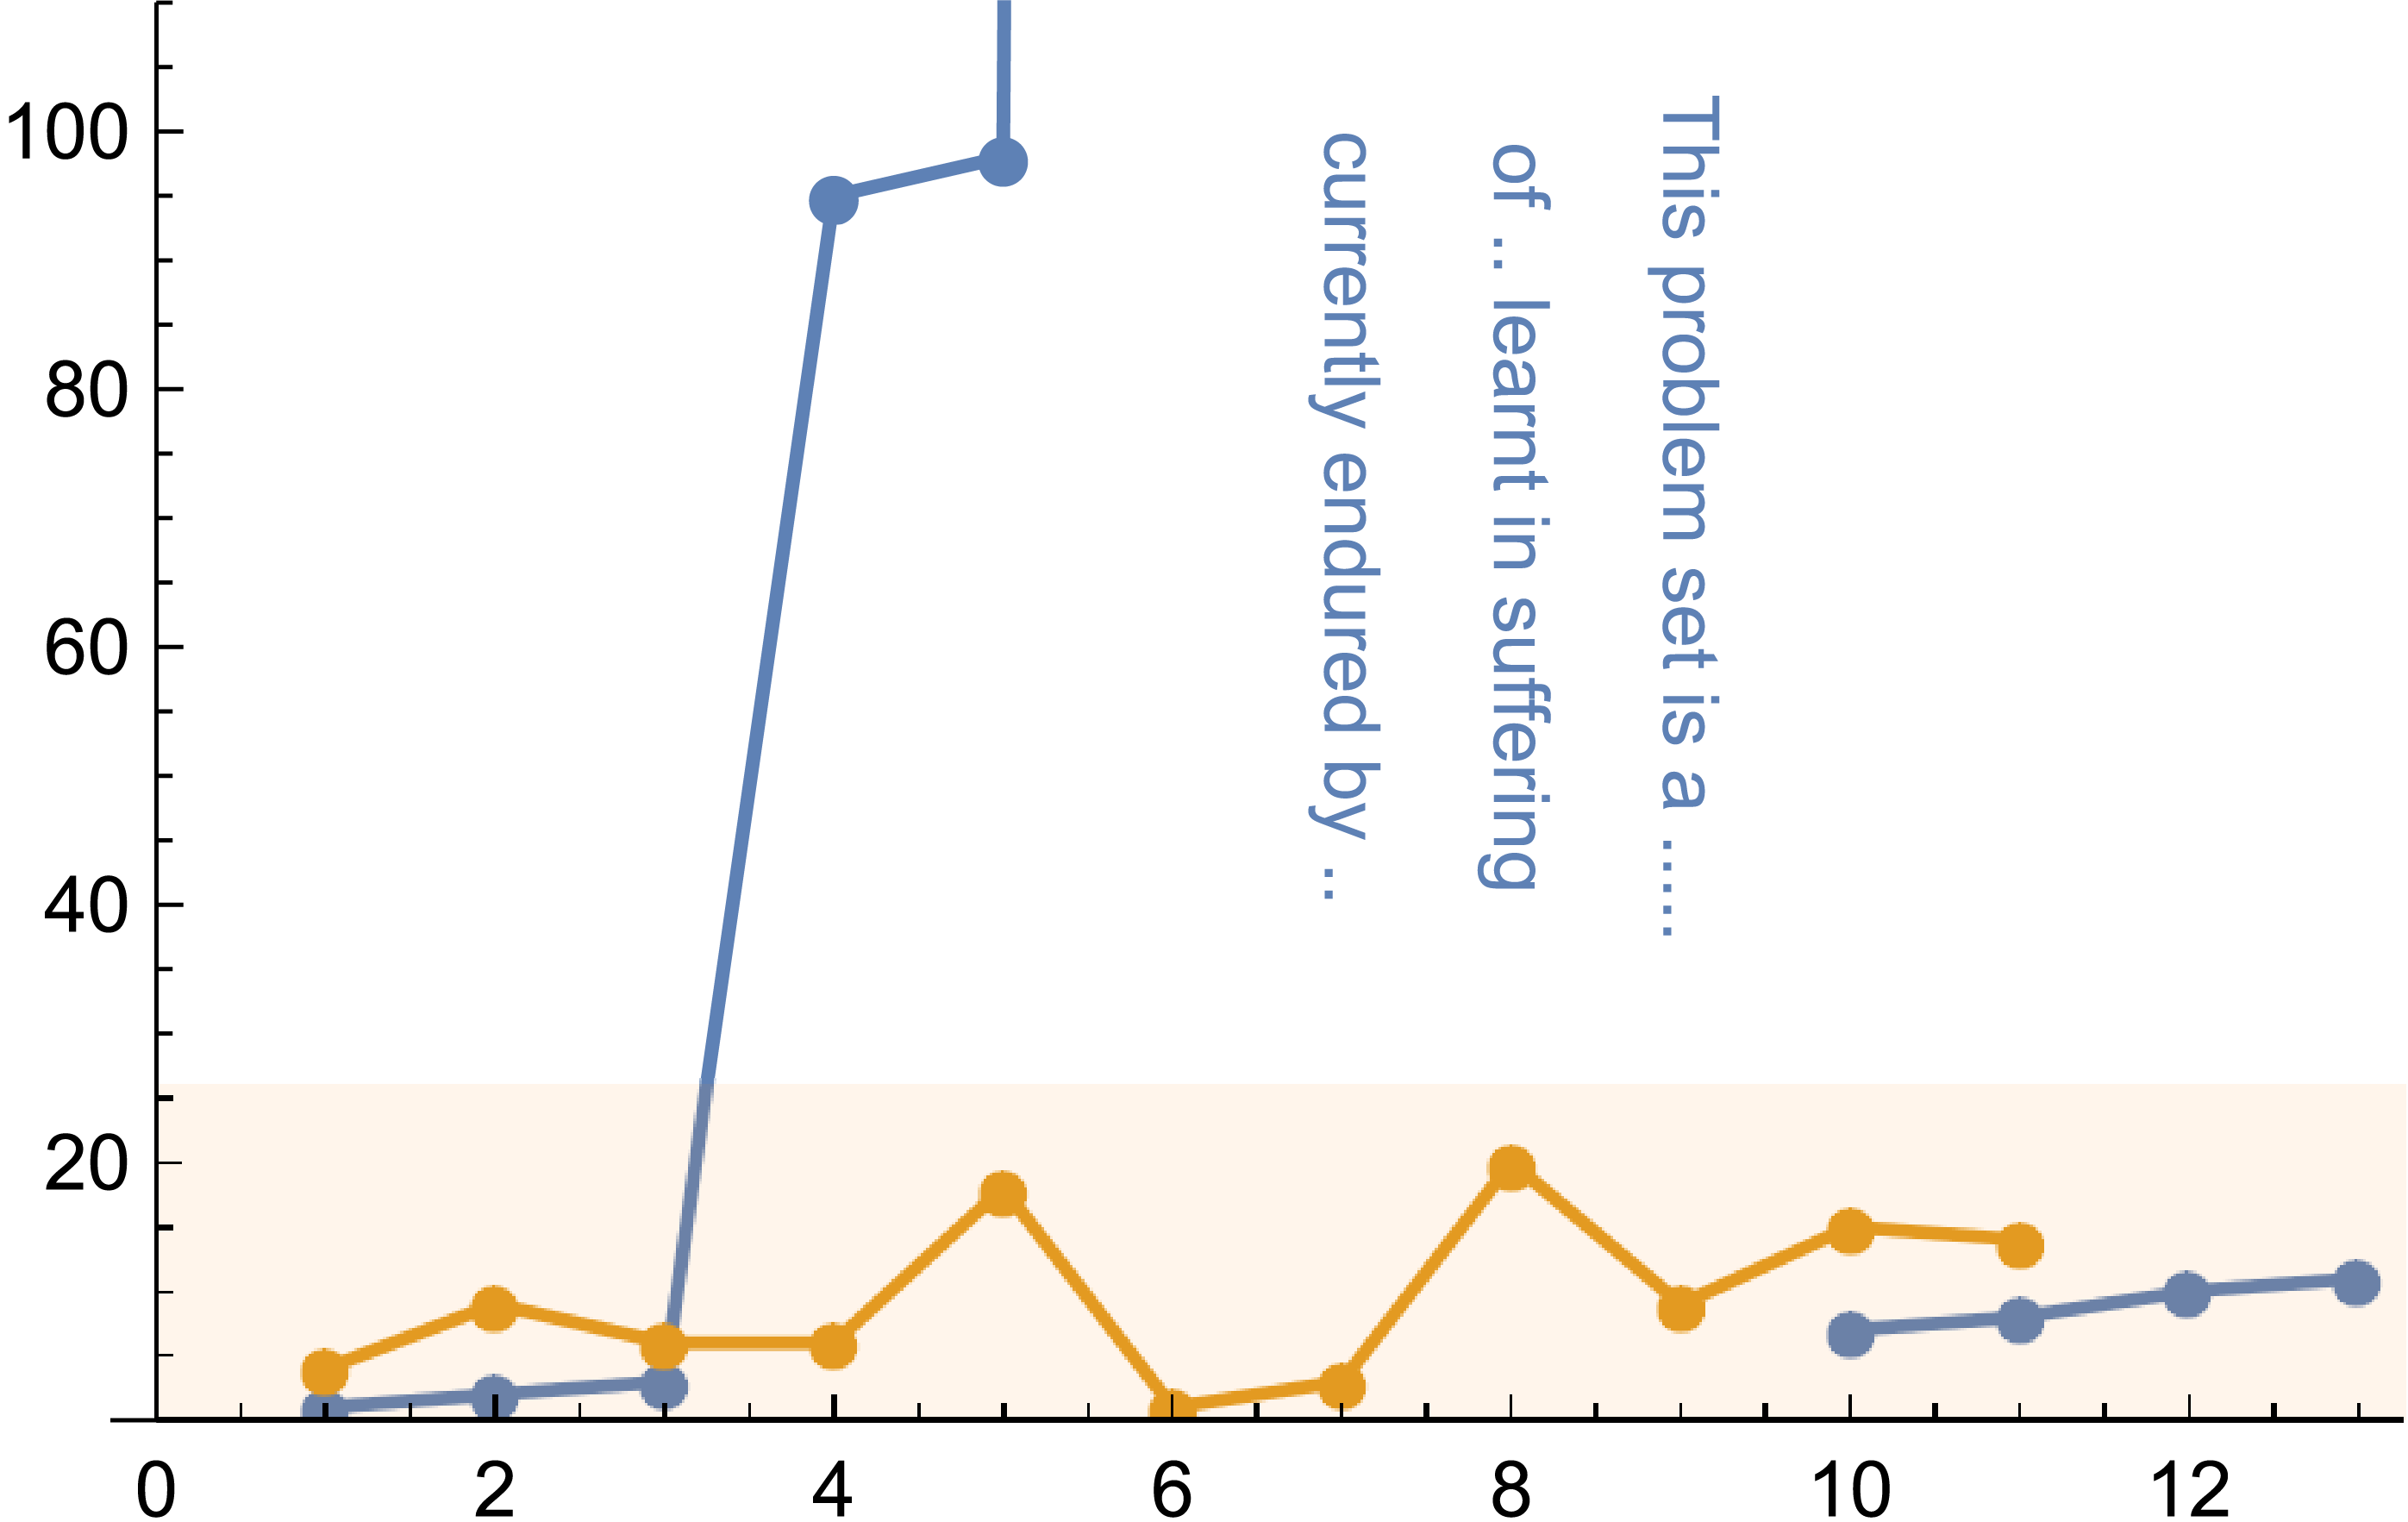
\includegraphics[width=0.67\columnwidth]{0.png}
		
		\small{\textit{(modified from \href{https://ccbc15.cipherpuzzles.com/info/about}{Cipher \& Code Breaking Competition 15})}}
	\end{figure}
	\vspace*{\fill}
	
	
	\setcounter{page}{0}
	
	\newpage
	
	\noindent
	\textbf{题一:真的有几十特斯拉的磁场吗?(Is There Really a Magnetic Field of Tens of Tesla?)}
	
	(1)(25分)
	
	正负带电粒子受到的保守力可以由势能对相应的坐标求导得出,即
	\begin{equation}\label{E1-01}
		\vec F_i=-\frac{1}{N_c}\frac{\partial V}{\partial \vec R}=-m_i\Omega_i^2\vec R-\delta\vec \rho
	\end{equation}
	\begin{equation}\label{E1-02}
		\vec F_e=-\frac{1}{N_c}\frac{\partial V}{\partial \vec\rho}=-m_e\Omega_e^2\vec \rho-\delta\vec R
	\end{equation}
	
	考虑右旋圆偏振光的情形。光的电场强度随时间的变化为
	\begin{equation}\label{E1-03}
		\vec E(t)=E_R[\cos(\omega t)\hat x+\sin(\omega t)\hat y]
	\end{equation}
	
	受此电场激发时,在稳定状态下,两种带电粒子的运动(仅提取对应于角频率$\omega$的部分)应当为匀速圆周运动。其转动方向与$\vec E$的转动方向相同,且$\vec R$、$\vec\rho$与$\vec E$应当始终在同一直线上。假设正带电粒子的运动半径为$R_R$,负带电粒子的运动半径为$\rho_R$(正方向均取与$\vec E$相同)。结合\eqref{E1-01}\eqref{E1-02}式,根据牛顿第二定律
	\begin{equation}\label{E1-04}
		-m_i\Omega_i^2 R_R-\delta\rho_R+e E_R+eB\omega R_R=-m_i\omega^2R_R
	\end{equation}
	\begin{equation}\label{E1-05}
		-m_e\Omega_e^2\rho_R-\delta R_R-e E_R-eB\omega \rho_R=-m_e\omega^2\rho_R
	\end{equation}
	
	联立\eqref{E1-03}\eqref{E1-04}\eqref{E1-05}解得
	\begin{equation}\label{E1-06}
		R_R=\frac{e\left[m_e(\omega^2-\Omega_e^2)-eB\omega\right]-e\delta}{\delta^2-\left[m_e(\omega^2-\Omega_e^2)-eB\omega\right]\left[m_i(\omega^2-\Omega_i^2)+eB\omega\right]}E_R
	\end{equation}
	\begin{equation}\label{E1-07}
		\rho_R=\frac{e\delta-e\left[m_i(\omega^2-\Omega_i^2)+eB\omega\right]}{\delta^2-\left[m_e(\omega^2-\Omega_e^2)-eB\omega\right]\left[m_i(\omega^2-\Omega_i^2)+eB\omega\right]}E_R
	\end{equation}
	
	根据电极化强度的定义
	\begin{equation}\label{E1-08}
		P_R=\chi_RE_R=N_ce(R_R-\rho_R)
	\end{equation}
	
	联立\eqref{E1-06}\eqref{E1-07}\eqref{E1-08}可得
	\begin{equation}\label{E1-09}
		\chi_R=\frac{N_ce^2\left[m_e(\omega^2-\Omega_e^2)+m_i(\omega^2-\Omega_i^2)-2\delta\right]}{\delta^2-\left[m_e(\omega^2-\Omega_e^2)-eB\omega\right]\left[m_i(\omega^2-\Omega_i^2)+eB\omega\right]}
	\end{equation}
	
	同理,对于左旋圆偏振光
	\begin{equation}\label{E1-10}
		\chi_L=\frac{N_ce^2\left[m_e(\omega^2-\Omega_e^2)+m_i(\omega^2-\Omega_i^2)-2\delta\right]}{\delta^2-\left[m_e(\omega^2-\Omega_e^2)+eB\omega\right]\left[m_i(\omega^2-\Omega_i^2)-eB\omega\right]}
	\end{equation}
	
	结合$\Delta\varepsilon$很小,展开至$B$的一阶小量,得到
	\begin{equation}\label{E1-11}
		\begin{aligned}
			\Delta\varepsilon&=\varepsilon_R-\varepsilon_L=\chi_R-\chi_L\\
			&\approx\frac{2N_ce^3\omega\left[m_e(\omega^2-\Omega_e^2)+m_i(\omega^2-\Omega_i^2)-2\delta\right]\left[m_e(\omega^2-\Omega_e^2)-m_i(\omega^2-\Omega_i^2)\right]}{\left[\delta^2-m_e(\omega^2-\Omega_e^2)m_i(\omega^2-\Omega_i^2)\right]^2}B
		\end{aligned}
	\end{equation}
	
	根据折射率的表达式
	\begin{equation}\label{E1-12}
		n=\sqrt{\frac{\varepsilon}{\varepsilon_0}},\,\Delta n=\frac{1}{2n(\omega)}\frac{\Delta\varepsilon}{\varepsilon_0}
	\end{equation}
	
	联立\eqref{E1-11}\eqref{E1-12}可得
	\begin{equation}\label{E1-13}
		\Delta n=\frac{N_ce^3\omega\left[m_e(\omega^2-\Omega_e^2)+m_i(\omega^2-\Omega_i^2)-2\delta\right]\left[m_e(\omega^2-\Omega_e^2)-m_i(\omega^2-\Omega_i^2)\right]}{n(\omega)\varepsilon_0\left[\delta^2-m_e(\omega^2-\Omega_e^2)m_i(\omega^2-\Omega_i^2)\right]^2}B
	\end{equation}
	
	由于折射率的差异,导致右旋圆偏振光和左旋圆偏振光之间的相位差异
	\begin{equation}
		\phi=\frac{\Delta n L}{c/\omega}=\frac{\omega L}{c}\Delta n
	\end{equation}
	
	因此,线偏振光的偏振面旋转角
	\begin{equation}\label{E1-15}
		\theta=\frac{\phi}{2}=\frac{\omega L}{2 c}\Delta n
	\end{equation}
	
	联立\eqref{E1-13}\eqref{E1-15}可得
	\begin{equation}
		\theta=\frac{N_ce^3\omega^2\left[m_e(\omega^2-\Omega_e^2)+m_i(\omega^2-\Omega_i^2)-2\delta\right]\left[m_e(\omega^2-\Omega_e^2)-m_i(\omega^2-\Omega_i^2)\right]}{2cn(\omega)\varepsilon_0\left[\delta^2-m_e(\omega^2-\Omega_e^2)m_i(\omega^2-\Omega_i^2)\right]^2}BL
	\end{equation}
	
	即
	\begin{equation}\label{E1-17}
		S(\omega)=\frac{N_ce^3\omega^2\left[m_e(\omega^2-\Omega_e^2)+m_i(\omega^2-\Omega_i^2)-2\delta\right]\left[m_e(\omega^2-\Omega_e^2)-m_i(\omega^2-\Omega_i^2)\right]}{2cn(\omega)\varepsilon_0\left[\delta^2-m_e(\omega^2-\Omega_e^2)m_i(\omega^2-\Omega_i^2)\right]^2}
	\end{equation}
	
	(2)(15分)
	
	假设正带电粒子的运动半径为$R_0$,负带电粒子的运动半径为$\rho_0$(正方向均取与$\vec E$相同)。参考\eqref{E1-04}\eqref{E1-05}式,运动方程为
	\begin{equation}
		-m_i\Omega_i^2 R_0-\delta\rho_0+e E_0=-m_i\omega^2R_0
	\end{equation}
	\begin{equation}
		-m_e\Omega_e^2\rho_0-\delta R_0-e E_0=-m_e\omega^2\rho_0
	\end{equation}
	
	解得
	\begin{equation}\label{E1-20}
		R_0=\frac{e\left[m_e(\omega^2-\Omega_e^2)-\delta\right]}{\delta^2-m_e(\omega^2-\Omega_e^2)m_i(\omega^2-\Omega_i^2)}E_0
	\end{equation}
	\begin{equation}\label{E1-21}
		\rho_0=\frac{e\left[\delta-m_i(\omega^2-\Omega_i^2)\right]}{\delta^2-m_e(\omega^2-\Omega_e^2)m_i(\omega^2-\Omega_i^2)}E_0
	\end{equation}
	
	结合磁化强度(单位体积内的磁矩)的表达式
	\begin{equation}\label{E1-22}
		M=N_c(e\omega R_0^2-e\omega\rho_0^2)
	\end{equation}
	
	联立\eqref{E1-20}\eqref{E1-21}\eqref{E1-22}得到
	\begin{equation}
		\begin{aligned}
			M&=\frac{N_ce^3\omega\left(\left[m_e(\omega^2-\Omega_e^2)-\delta\right]^2-\left[\delta-m_i(\omega^2-\Omega_i^2)\right]^2\right)}{\left[\delta^2-m_e(\omega^2-\Omega_e^2)m_i(\omega^2-\Omega_i^2)\right]^2}E_0^2\\
			&=\frac{N_ce^3\omega\left[m_e(\omega^2-\Omega_e^2)+m_i(\omega^2-\Omega_i^2)-2\delta\right]\left[m_e(\omega^2-\Omega_e^2)-m_i(\omega^2-\Omega_i^2)\right]}{\left[\delta^2-m_e(\omega^2-\Omega_e^2)m_i(\omega^2-\Omega_i^2)\right]^2}E_0^2
		\end{aligned}
	\end{equation}
	
	所以
	\begin{equation}\label{E1-24}
		T(\omega)=\frac{N_ce^3\omega\left[m_e(\omega^2-\Omega_e^2)+m_i(\omega^2-\Omega_i^2)-2\delta\right]\left[m_e(\omega^2-\Omega_e^2)-m_i(\omega^2-\Omega_i^2)\right]}{\left[\delta^2-m_e(\omega^2-\Omega_e^2)m_i(\omega^2-\Omega_i^2)\right]^2}
	\end{equation}
	
	比较\eqref{E1-17}和\eqref{E1-24}可得
	\begin{equation}
		T(\omega)=\frac{2cn(\omega)\varepsilon_0}{\omega}S(\omega)
	\end{equation}
	
	(3)(4分)
	
	代入数据($\omega=\omega_0$)至\eqref{E1-20}\eqref{E1-21}式,得到
	\begin{equation}\label{E1-26}
		|R_0|=9.2\times10^{-13}\,\text{m},\,|\rho_0|=3.1\times10^{-11}\,\text{m}
	\end{equation}
	
	利用\eqref{E1-22}式,结合$B=\mu_0 M$,得到(以$z$轴正方向为正)
	\begin{equation}\label{E1-27}
		B=\mu_0 M=-2.9\times10^{-4}\,\text{T}
	\end{equation}
	
	代入数据($\omega=\omega_1$)至\eqref{E1-17}式,得到
	\begin{equation}\label{E1-28}
		S(\omega_1)=-1.1\times10^2\,\text{T}^{-1}\text{m}^{-1}
	\end{equation}
	
	综合\eqref{E1-27}\eqref{E1-28}可得
	\begin{equation}
		\theta_F=S(\omega_1)BL=3.2\times10^{-7}\,\text{rad}
	\end{equation}
	
	(4.1)(7分)
	
	能量项$\kappa\rho_x^3$对应的力为
	\begin{equation}\label{E1-30}
		F_{\kappa}=-\frac{\partial\Delta V}{\partial\rho_x}=-3\kappa\rho_x^2
	\end{equation}
	
	因为$3\kappa\rho_0^2\ll |m_e(\omega_0^2-\Omega_e^2)\rho_0|$,所以可以将上述与$\kappa$成正比的项当作微扰。在原有运动轨迹(匀速圆周运动)的一个周期内,该项的期望值为
	\begin{equation}\label{E1-31}
		\langle F_{\kappa}\rangle=-\frac{3\kappa\rho_0^2}{2\pi}\int_{0}^{2\pi}(\cos\theta)^2\ud\theta=-\frac{3\kappa\rho_0^2}{2}
	\end{equation}
	
	可以估算轨迹中心的位移大小为
	\begin{equation}\label{E1-32}
		\rho_{\kappa}=\frac{|\langle F_{\kappa}\rangle|}{|m_e(\omega_0^2-\Omega_e^2)|}=\frac{3\kappa\rho_0^2}{2|m_e(\omega_0^2-\Omega_e^2)|}=1.4\times10^{-12}\,\text{m}
	\end{equation}
	
	(4.2)(3分)
	
	由$\rho_{\kappa}$所导致的对正带电粒子的作用力为
	\begin{equation}\label{E1-33}
		F_{\delta,\kappa}=-\delta\rho_{\kappa}
	\end{equation}
	
	可以估算轨迹中心的位移大小为
	\begin{equation}\label{E1-34}
		R_{\kappa}=\frac{|F_{\delta,\kappa}|}{|m_i(\omega_0^2-\Omega_i^2)|}=\frac{\delta\rho_{\kappa}}{|m_i(\omega_0^2-\Omega_i^2)|}=1.9\times10^{-15}\,\text{m}
	\end{equation}
	
	(4.3)(6分)
	
	正带电粒子在势场中的位置可以分解为$\vec R=\vec R^{(0)}+\vec R_{\kappa}$,其中$\vec R^{(0)}$是未受微扰时的圆周运动的位移。由于在一个周期内,$\vec R^{(0)}\cdot\vec R_{\kappa}$的平均值为零,所以可以估计一个正带电粒子由于运动轨迹偏移所导致的能量变化的绝对值为
	\begin{equation}\label{E1-35}
		u_{\kappa}=\frac{m_i\Omega_i^2}{2}R_{\kappa}^2
	\end{equation}
	
	而在另一种情形下,一个正带电粒子粒子在假想磁场$B_{eff}$中的磁能的绝对值
	\begin{equation}\label{E1-36}
		u_{eff}=e\omega R_0^2 |B_{eff}|
	\end{equation}
	
	由题设$u_{eff}=u_{\kappa}$,结合\eqref{E1-35}\eqref{E1-36}可得
	\begin{equation}
		|B_{eff}|=\frac{m_i\Omega_i^2R_{\kappa}^2}{2e\omega R_0^2}=49\,\text{T}
	\end{equation}
	
	这一等效磁场$|B_{eff}|$比(3)中算出的真实磁场$|B|$大五个数量级。
	
		
	也可用$\rho_{\kappa}=3\kappa\rho_0^2/(2m_e\Omega_e^2)$和$R_{\kappa}=\delta\rho_{\kappa}/(m_i\Omega_i^2)$估计,得到$|B_{eff}|=10\,\text{T}$。其他相差量级为1的常数的估算方法也对。\\
	
	【说明1】在$\omega$满足或接近共振条件时,(2)问中的结果可能会远离物理实际,因为此时必须考虑粒子运动时的阻尼。如果认为阻力与速度方向相反且大小成正比,则$\vec r,\vec\rho,\vec E$可以不在同一条直线上,但稳定时三者仍然以相同的角速度转动,原则上仍然可以求解,只是表达式更复杂了。
	
	【说明2】个人对这个问题的图像上的理解:在线性近似下(势能是坐标的二阶项),晶体中角频率为$\omega_0$(圆偏振光)和角频率为$\omega_1$(线偏振光)的运动是不会相互影响的。如果直接采用$\theta_E=S(\omega_1)LB$反推出$B$,相当于认为上述影响的主要途径是通过圆偏振光产生的磁场,然后磁场再作用于带电粒子的运动。然而,一般的顺磁性材料中这样的相互作用的效率是非常低的(作为估算,可以认为是磁化率$\chi\sim10^{-5}$的量级)。而如果带电粒子运动时感受到的势能本身是非线性的,不同频率的运动就能以$\sim0.1$的效率耦合,远远高于通过磁场进行耦合的效率。因此,如果错误地假设主要的耦合形式来源于磁场,理论预期就会与实验结果有$\sim10^4$的差异。
	
	\setcounter{equation}{0}
	
	\newpage
	
	\noindent
	\textbf{题二:动量是否守恒?(Is Momentum Conserved?)}
	
	(1)(13分)
	
	首先将$V_p(d)$写成等效的对应每对正负电荷$\pm Q$的形式。平均每对正负离子占据的体积为
	\begin{equation}\label{E2-01}
		V_0=\frac{(2a)^3}{4}=2a^3
	\end{equation}
	
	因此,对应于每对正负离子的晶体内势能形式为
	\begin{equation}\label{E2-02}
		V(d)=\frac{1}{V_0}V_p(d)=\frac{\zeta}{2a^3}d^2
	\end{equation}
	
	相应于每个离子受到的回复力
	\begin{equation}\label{E2-03}
		F(d)=-V'(d)=-\frac{\zeta}{a^3}d
	\end{equation}
	负号表示其方向与位移$\vec d$相反。
	
	当$\omega=0$时,即外加电场是静电场时,设此时A离子相对B离子的位移为$d_m$,则根据力平衡条件
	\begin{equation}\label{E2-04}
		\vec F(\vec d_m)+Q\vec E=0
	\end{equation}
	
	联立\eqref{E2-03}\eqref{E2-04}得
	\begin{equation}\label{E2-05}
		\vec{d}_m=\frac{Qa^3}{\zeta}\vec E
	\end{equation}
	
	一对正负离子对应的电偶极矩为$\vec p_m=Q\vec{d}_m$,对应的电极化强度为
	\begin{equation}\label{E2-06}
		\vec P_m=\frac{\vec p_m}{V_0}=\frac{Q}{2a^3}\vec d_m
	\end{equation}
	
	由题文,知$\vec{P}=\chi\vec E+\vec P_m$。结合\eqref{E2-05}\eqref{E2-06}得
	\begin{equation}\label{E2-07}
		\vec{P}_{st}=\left(\chi+\frac{Q^2}{2\zeta}\right)\vec E
	\end{equation}
	
	结合电位移矢量的定义$\vec D=\varepsilon_0\vec E+\vec P=\varepsilon\vec E$得到
	\begin{equation}\label{E2-08}
		\varepsilon_{st}=\chi+\frac{Q^2}{2\zeta}+\varepsilon_0
	\end{equation}
	
	当$\omega$很大时,离子实的运动跟不上电场的变化,因此电极化强度只有电场的贡献$\vec P=\vec P_e$。故
	\begin{equation}\label{E2-09}
		\varepsilon_{\infty}=\chi+\varepsilon_0
	\end{equation}
	
	(2.1)(3分)
	
	晶体中任意部分不出现宏观运动即对任意$x,y,z,t$,都有
	\begin{equation}\label{E2-10}
		m_A\vec r_A(x,y,z,t)+m_B\vec r_B(x,y,z,t)\equiv0
	\end{equation}
	故$m_A\vec R_A+m_B\vec R_B=0$,或$\vec R_B=-m_A\vec R_A/m_B$。
	
	(2.2)(11分)
	
	考虑两种离子相对质心的运动,定义$\vec r=\vec r_A-\vec r_B=\vec R\ue^{\ui(kz-\omega t)}$。由$k\ll 1/a$,在某一对离子附近的离子实分布同定义$V_p$时的情形区别很小,回复力仍可近似为$F(\vec r)$。结合电场项,其运动方程为
	\begin{equation}\label{E2-11}
		m\ddot{\vec r}=F(\vec r)+Q\vec E
	\end{equation}
	其中约化质量$m=m_Am_B/(m_A+m_B)$。$F(\vec r)$由\eqref{E2-03}给出,即
	\begin{equation}\label{E2-12}
		m\ddot{\vec r}=-\frac{\zeta}{a^3}\vec r+Q\vec E
	\end{equation}
	
	参考(1)中的推导,可得电极化强度的表达式
	\begin{equation}\label{E2-13}
		\vec P=\chi\vec E+\frac{Q}{2a^3}\vec r
	\end{equation}
	
	电位移矢量的表达式为
	\begin{equation}\label{E2-14}
		\vec D=\vec P+\varepsilon_0\vec E=(\chi+\varepsilon_0)\vec E+\frac{Q}{2a^3}\vec r
	\end{equation}
	
	代入$\vec D=0$,得到
	\begin{equation}\label{E2-15}
		\vec{E}=-\frac{Q}{2a^3(\chi+\varepsilon_0)}\vec r
	\end{equation}
	
	代回\eqref{E2-12}式,得到
	\begin{equation}\label{E2-16}
		m\ddot{\vec r}=-\left(\frac{\zeta}{a^3}+\frac{Q^2}{2a^3(\chi+\varepsilon_0)}\right)\vec r
	\end{equation}
	
	因此对应的频率与$k$无关,为
	\begin{equation}\label{E2-17}
		\nu_{LO}=\frac 1 {2\pi}\sqrt{\frac{(m_A+m_B)}{m_Am_B}\left(\frac{\zeta}{a^3}+\frac{Q^2}{2a^3(\chi+\varepsilon_0)}\right)}
	\end{equation}
	
	(2.3)(16分)
	
	将\eqref{E2-14}式代入$\vec D$和$\vec E$的关系,得到
	\begin{equation}\label{E2-18}
		k^2\vec{E}=\omega^2\mu_0\left[(\chi+\varepsilon_0)\vec E+\frac{Q}{2a^3}\vec r\right]
	\end{equation}
	
	联立\eqref{E2-12}\eqref{E2-18}得
	\begin{equation}\label{E2-19}
		m\ddot{\vec r}=-\frac{\zeta}{a^3}\vec r+\frac{\omega^2\mu_0Q^2}{2a^3\left[k^2-\omega^2\mu_0(\chi+\varepsilon_0)\right]}\vec r
	\end{equation}
	
	即
	\begin{equation}\label{E2-20}
		\omega^2=\frac{1}{m}\left(\frac{\zeta}{a^3}-\frac{\omega^2\mu_0Q^2}{2a^3\left[k^2-\omega^2\mu_0(\chi+\varepsilon_0)\right]}\right)
	\end{equation}
	
	解得
	\begin{multline}\label{E2-21}
		\omega^2_{\pm}(k)=\frac{\zeta(m_A+m_B)}{2m_Am_Ba^3}+\frac{k^2}{2\mu_0(\chi+\varepsilon_0)}+\frac{(m_A+m_B)Q^2}{4m_Am_Ba^3(\chi+\varepsilon_0)}\\ \pm\sqrt{\left(\frac{\zeta(m_A+m_B)}{2m_Am_Ba^3}+\frac{k^2}{2\mu_0(\chi+\varepsilon_0)}+\frac{(m_A+m_B)Q^2}{4m_Am_Ba^3(\chi+\varepsilon_0)}\right)^2-\frac{(m_A+m_B)\zeta k^2}{2m_Am_Ba^3\mu_0(\chi+\varepsilon_0)}}
	\end{multline}
	
	对于$\omega_+$,在$k$很大时,$\omega_+^2$的首阶非零项正比于$k^2$,即
	\begin{equation}\label{E2-22}
		\omega^2_+\approx\frac{k^2}{\mu_0(\chi+\varepsilon_0)},\,\omega_+\approx\frac{k}{\sqrt{\mu_0(\chi+\varepsilon_0)}}
	\end{equation}
	
	在$k$很大时,根式中的后一项远小于前一项。利用展开式$\sqrt{1-x}\approx 1-x/2,\,x\ll1$,得到
	\begin{equation}\label{E2-23}
		\omega_-^2\approx\frac{(m_A+m_B)\zeta }{m_Am_Ba^3},\,\omega_-\approx\sqrt{\frac{(m_A+m_B)\zeta }{m_Am_Ba^3}}
	\end{equation}
	
	因此
	\begin{equation}\label{E2-24}
		\nu_{TO}=\frac 1 {2\pi}\sqrt{\frac{(m_A+m_B)\zeta }{m_Am_Ba^3}}
	\end{equation}
	
	(2.4)(9分)
	
	联立\eqref{E2-08}\eqref{E2-09}\eqref{E2-17}\eqref{E2-24}可得
	\begin{equation}
		\nu_{LO}=\nu_{TO}\sqrt{\frac{\varepsilon_{st}}{\varepsilon_{\infty}}}
	\end{equation}
	代入数据得到$\nu_{LO}=7.9\times10^{12}\,\text{Hz}$。
	
	计算一些画图需要的关键信息:
	
	(i)当$k$很大时,$\omega_+\approx ck/(\sqrt{\varepsilon_{\infty}/\varepsilon_0})$;
	
	(ii)直线$\omega=\omega_{LO}$与$\omega= ck/(\sqrt{\varepsilon_{\infty}/\varepsilon_0})$的交点为$k=1.6\times10^{-4}\,\text{nm}^{-1}\sim10^{-5}a^{-1}$。(所以上述讨论中$k$很大的极限值是可以在满足$k\ll1/a$的情况下取到的。)
	
	(iii)当$k=0$时,$\omega_+=\omega_{LO}$而$\omega_-=0$。
	
	\begin{figure}[!bh]
		\centering
		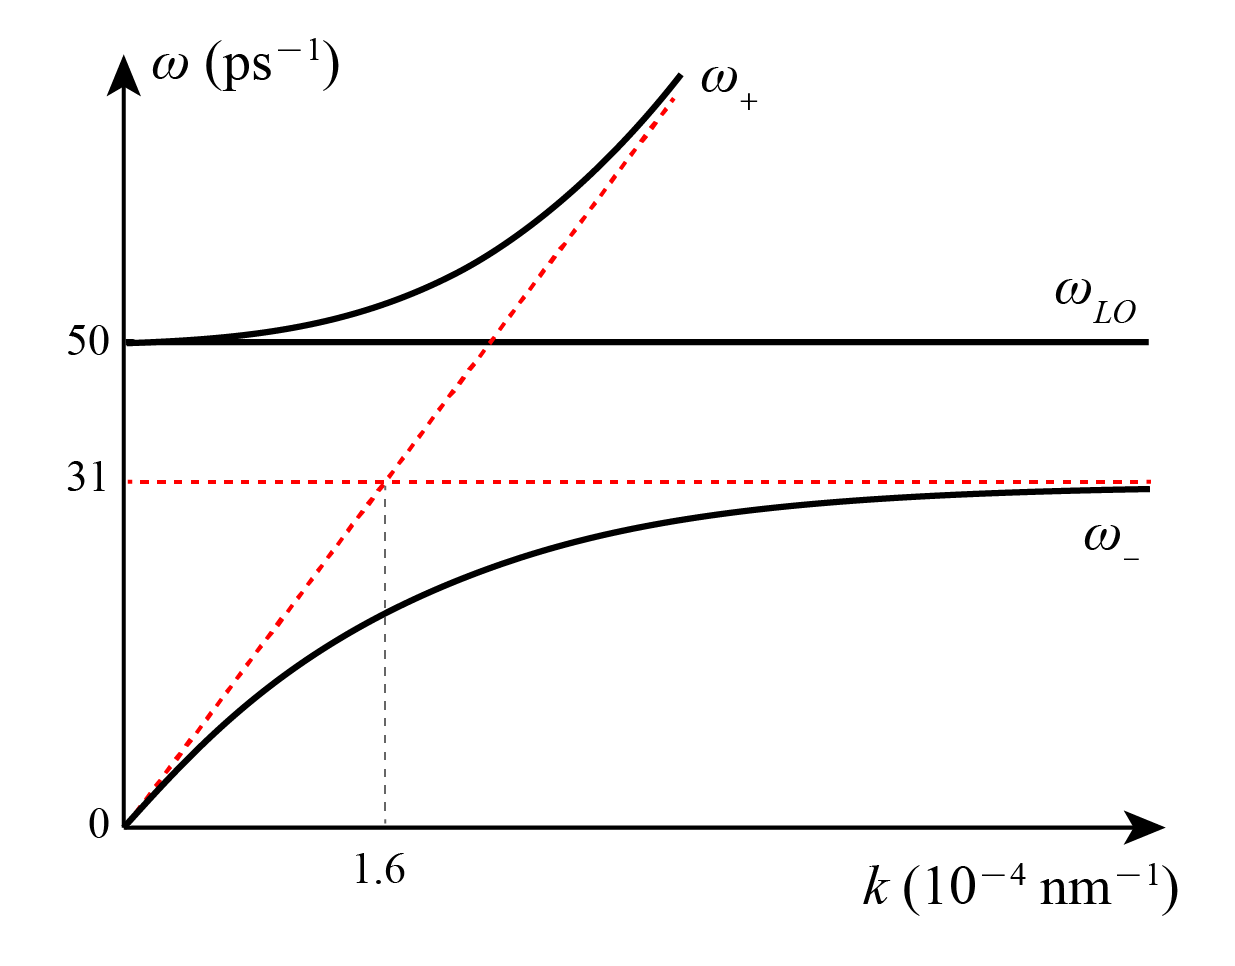
\includegraphics[width=0.6\columnwidth]{FA.png}
	\end{figure}
	
	(3)(8分)
	
	$\omega$必须等于$\omega_l$,因为在一个光子产生一个极化子的过程中能量守恒(也可从相因子$\ue^{-\ui\omega t}$和$\ue^{-\ui\omega_l t}$的角度考虑)。
	
	$k$不必须等于$k_l$,因为垂直于样品表面的方向上平移对称性被破缺,不满足动量守恒的条件(也可从相因子$\ue^{\ui k z}$在表面上是常数的角度考虑)。
	
	激发效率正比于$\omega_l$到$\omega_l+\ud\omega_l$中的量子态数目,也正比于与该频率范围对应的波矢$k$的可取范围。当$\omega_l\to\omega_{TO}$时,对应极化子波矢$k$的可取范围最大,因而激发效率最高。(注意上面已经说明了$\omega(k)=\omega_{LO}$的分支是纵波,不能被电磁波直接激发。所以这里只需要考虑$\omega_{\pm}$对应的两支。)\\
	
	【说明】类似的关于极化子和纵光学声子的理论模型,在黄昆1951年的论文Lattice Vibrations and Optical Waves in Ionic Crystals (Nature 167 (4254): 779–780)中就有提及。
	
	
	
	\setcounter{equation}{0}
	\newpage

	\noindent
	\textbf{题三:研究物理不如研究机器学习(It is Better to Study Machine Learning Than Study Physics)}
	
	(1)(6分)
	
	参考系$S_1$是非惯性系,其中的加速度$\vec a_1$与惯性参考系中的加速度$\vec a_0$不同。两者的差异由非惯性系中的惯性力(惯性加速度)给出,其表达式为
	\begin{equation}\label{E3-01}
		\vec a_1-\vec a_0=\vec a_S+\vec\omega_S^2\vec r_{\perp}-2\vec\omega_S\times\frac{\ud \vec r_1}{\ud t}-\frac{\ud \vec\omega_S}{\ud t}\times\vec r_1
	\end{equation}
	其中$\vec a_S$是参考系$S_1$坐标原点在惯性系中的加速度,$\vec\omega_S$是参考系$S_1$的角速度,$\vec r_1$是$C$点在参考系$S_1$中的位矢,$\vec r_{\perp}$是$\vec r_1$在垂直于参考系$S_1$的转轴方向的投影。这几项惯性力分别是:平动惯性力、惯性离心力、科里奥利力、坐标系变速旋转导致的惯性力。
	
	(2)(22分)
	
	记
	$$R_0=\sqrt{\left(c+\sqrt{c^2-\left(b/2\right)^2}\right)^2+(b/2)^2}=60.39\,\text{cm}$$
	$$\theta_0=\arctan\left(\frac{b/2}{c+\sqrt{c^2-\left(b/2\right)^2}}\right)=0.3376$$
	
	则在$t=0$时刻,$C$点相对于$S_1$(或$S_0$)坐标原点的位矢为
	\begin{equation}\label{E3-02}
		\vec r_s=\left(h-H/2+R_0\cos\theta_0\right)\hat z_1
	\end{equation}
	
	在$S_1$(或$S_0$)参考系中的速度为
	\begin{equation}\label{E3-03}
		\vec v_s=\Omega_1R_0\left(\cos\theta_0\hat x_1+\sin\theta_0\hat z_1\right)
	\end{equation}	
	
	在任意时刻$t$,$C$点在$S_1$参考系中的位矢为
	\begin{equation}\label{E3-04}
		\vec r_1(t)=(b/2)\hat x_1+(h-H/2)\hat z_1+R_0\left(\sin(\Omega_1t-\theta_0)\hat x_1+\cos(\Omega_1t-\theta_0)\hat z_1\right)
	\end{equation}
	
	速度为
	\begin{equation}
		\vec v_1(t)=\Omega_1R_0\left(\cos(\Omega_1t-\theta_0)\hat x_1-\sin(\Omega_1t-\theta_0)\hat z_1\right)
	\end{equation}
	
	加速度为
	\begin{equation}
		\vec a_1(t)=-\Omega_1^2R_0\sin(\Omega_1t-\theta_0)\hat x_1-\Omega_1^2R_0\cos(\Omega_1t-\theta_0)\hat z_1
	\end{equation}
	
	将上述信息代入\eqref{E3-01}式中,并利用$\vec a_S=0$、$\vec \omega_S=\Omega_0\hat z_1$、$\ud\vec\omega_S/\ud t=0$,得到
	\begin{equation}\label{E3-07}
		\begin{aligned}
			\vec a_0(t)&=\vec a_1-\Omega_0^2\vec r_{\perp}+2\Omega_0\hat z_1\times \vec v_1\\
			&=-\left[(\Omega_0^2+\Omega_1^2)R_0\sin(\Omega_1t-\theta_0)+\Omega_0^2(b/2)\right]\hat x_1+2\Omega_0\Omega_1R_0\cos(\Omega_1t-\theta_0)\hat y_1\\&\,\,\,\,\,-\Omega_1^2R_0\cos(\Omega_1t-\theta_0)\hat z_1
		\end{aligned}
	\end{equation}
	
	据题设,若采用错误的算法,则计算出的$t$时刻在$S_1$参考系中的速度为
	\begin{equation}
		\vec v_1^{\star}(t)=\int_{0}^{t'}\vec a_0(t')\ud t+\vec v_s
	\end{equation}
	
	结合\eqref{E3-03}和\eqref{E3-07},得到
	\begin{equation}\label{E3-09}
		\begin{aligned}
			\vec v_1^{\star}(t)&=\left[\frac{\Omega_0^2+\Omega_1^2}{\Omega_1}R_0\cos(\Omega_1t-\theta_0)-\frac{\Omega_0^2}{\Omega_1}R_0\cos(\theta_0)-\Omega_0^2(b/2)t\right]\hat x_1\\
			&\,\,\,\,\,+2\Omega_0R_0\left[\sin(\Omega_1t-\theta_0)+\sin(\theta_0)\right]\hat y_1-\Omega_1R_0\sin(\Omega_1t-\theta_0)\hat z_1
		\end{aligned}
	\end{equation}
	
	错误的位置矢量是由$\vec v_1^{\star}$再次积分得到的,即
	\begin{equation}
		\vec r_1^{\star}(t)=\int_{0}^{t}\vec v_1^{\star}(t')\ud t'+\vec r_s
	\end{equation}
	
	结合\eqref{E3-02}和\eqref{E3-09},得到
	\begin{equation}\label{E3-11}
		\begin{aligned}
			\vec r_1^{\star}(t)&=\left[\frac{\Omega_0^2+\Omega_1^2}{\Omega_1^2}R_0\left(\sin(\Omega_1t-\theta_0)+\sin\theta_0\right)-\frac{\Omega_0^2}{\Omega_1}R_0\cos(\theta_0)t-\frac1 2\Omega_0^2(b/2)t^2\right]\hat x_1\\
			&\,\,\,\,\,+\left[2\frac{\Omega_0}{\Omega_1}R_0[\cos(\theta_0)-\cos(\Omega_1t-\theta_0)]+2\Omega_0R_0\sin(\theta_0)t\right]\hat y_1\\
			&\,\,\,\,\,+\left[R_0\cos(\Omega_1t-\theta_0)+h-H/2\right]\hat z_1
		\end{aligned}
	\end{equation}
	
	代入数据,得到位置矢量在$S_1$各坐标轴投影上的分量
	\begin{equation}
		\vec r_1^{\star}(\tau)=(0.385\,\text{m},0.808\,\text{m},1.10\,\text{m})
	\end{equation}
	
	代入数据至\eqref{E3-04}式,得到正确的结果
	\begin{equation}
		\vec r_1(\tau)=(0.571\,\text{m},0,1.10\,\text{m})
	\end{equation}
	
	因此,错误结果与正确结果之间的距离
	\begin{equation}
		|\vec r_1^{\star}-\vec r_1|=0.829\,\text{m}
	\end{equation}
	
	(3)(22分)
	
	在肘关节不动的情况下,手臂整体可以认为是一个刚体。计算$t=0$时刻该刚体的质心$G$相对$A$点的位置,得到
	\begin{equation}
		\begin{aligned}
			\overrightarrow{AG}&=\frac{1}{3}\left[-\frac b 4 \hat x_1+\left(c+\frac 1 2\left(c+\sqrt{c^2-\left(b/2\right)}\right)\right)\hat z_1\right]+\frac 2 3 (c/2)\hat z_1\\
			&=-\frac{b}{12}\hat x_1+\left(\frac c 2+\frac 1 6\left(c+\sqrt{c^2-\left(b/2\right)}\right)\right)\hat z_1
		\end{aligned}
	\end{equation}
	
	可采用与导出\eqref{E3-07}式相同的方法计算质心$G$在任意时刻$t$在惯性系中的加速度。这里我们只关心$y_1$方向的分量,即
	\begin{equation}\label{E3-16}
		a_{G,y1}=2\Omega_0\Omega_1R_G\cos(\Omega_1t-\theta_G)
	\end{equation}
	其中
	$$R_G=\sqrt{\left(\frac c 2+\frac 1 6\left(c+\sqrt{c^2-\left(b/2\right)}\right)\right)^2+(b/12)^2}=25.71\,\text{cm}$$
	$$\theta_G=\arctan\left(\frac{b/12}{c/2+\left(c+\sqrt{c^2-\left(b/2\right)}\right)/6}\right)=0.1300$$
	
	根据质心运动定理,肩关节对大臂作用力的$y_1$分量
	\begin{equation}\label{E3-17}
		F_{y1}=3ma_{G,y1}(\tau/2)
	\end{equation}
	
	联立\eqref{E3-16}\eqref{E3-17}并代入数据得
	\begin{equation}\label{E3-18}
		F_{y1}=2.66\,\text{N}
	\end{equation}
	
	下面考虑手臂绕过身体中心的竖直轴的角动量$L_z$。易知手臂在竖直平面内的运动对其没有贡献,因此只需求任意时刻$t$手臂相对于该转轴的转动惯量,再乘以$\Omega_0$即可。根据平行轴定理,大臂的转动惯量
	\begin{equation}\label{E3-19}
		I_{AB}(t)=\frac{2m}{12}(c\sin(\Omega_1t))^2+2m\left(\frac b 2+\frac c 2\sin(\Omega_1t)\right)^2
	\end{equation}
	
	小臂的转动惯量
	\begin{equation}\label{E3-20}
		I_{BC}(t)=\frac{m}{12}(c\sin(\Omega_1t-\phi))^2+m\left(\frac b 2+c\sin(\Omega_1t)+\frac c 2\sin(\Omega_1t-\phi)\right)^2
	\end{equation}
	
	其中$\phi=\arcsin(b/(2c))=0.6751$是大臂$AB$方向与小臂$BC$方向之间的夹角。角动量$L_z$可以表示为
	\begin{equation}\label{E3-21}
		L_z(t)=(I_{AB}(t)+I_{BC}(t))\Omega_0
	\end{equation}
	
	联立\eqref{E3-19}\eqref{E3-20}\eqref{E3-21},得到
	\begin{multline}\label{E3-22}
		\frac{\ud L_z}{\ud t}=\frac{mc^2\Omega_0\Omega_1}{12}\left[2\sin(2\Omega_1t)+\sin(2\Omega_1t-2\phi)\right]+2mc\Omega_0\Omega_1\left(\frac b 2+\frac c 2\sin(\Omega_1t)\right)\cos(\Omega_1t)\\+mc\Omega_0\Omega_1\left(\frac b 2+c\sin(\Omega_1t)+\frac c 2\sin(\Omega_1t-\phi)\right)\left(2\cos(\Omega_1t)+\cos(\Omega_1t-\phi)\right)
	\end{multline}
	
	相对于过身体中心的竖直轴,列出$z_1$方向的角动量定理
	\begin{equation}\label{E3-23}
		M_{z1}+\frac b 2F_{y1}=\left.\frac{\ud L_z}{\ud t}\right|_{t=\tau/2}
	\end{equation}
	
	联立\eqref{E3-18}\eqref{E3-22}\eqref{E3-23}并代入数据得
	\begin{equation}
		M_{z1}=0.304\,\text{N}\cdot\text{m}
	\end{equation}\\
	
	【注】特别地,上述解答不包含本题中的一个彩蛋问题(对应的分数为$20\ui$)。
	
	
	\setcounter{equation}{0}
	\newpage
	
	\noindent
	\textbf{题四:多次反射如何相加?(How to Add Up Multiple Reflections?)}
	
	(1)(6分)
	
	考虑到半波损失,干涉相长的条件为($m$为正整数)
	\begin{equation}
		2\Re(\tilde{n}_B)\sigma=(m-1/2)\lambda
	\end{equation}
	
	即
	\begin{equation}
		\lambda=\frac{3.90\times10^{5}\,\text{nm}}{m-1/2}
	\end{equation}
	
	干涉相消的条件为($m$为正整数)
	\begin{equation}
		2\Re(\tilde{n}_B)\sigma=m\lambda
	\end{equation}
	
	即
	\begin{equation}
		\lambda=\frac{3.90\times10^{5}\,\text{nm}}{m}
	\end{equation}
	
	
	(2)(15分)
	
	在真空--B界面,当光从真空入射时,反射光与入射光的复振幅之比为
	\begin{equation}\label{E4-01}
		\tilde r_1=\frac{1-\tilde n_B}{1+\tilde n_B}
	\end{equation}
	
	当光从B介质入射时的对应值是上述值取负号,即
	\begin{equation}\label{E4-02}
		\tilde{r}_2=-\tilde r_1=\frac{\tilde n_B-1}{1+\tilde n_B}
	\end{equation}
	
	当光从真空入射时,透射光与入射光的复振幅之比为
	\begin{equation}\label{E4-03}
		\tilde t_1=\frac{2}{1+\tilde n_B}
	\end{equation}
	
	当光从介质B入射时,透射光与入射光的复振幅之比为
	\begin{equation}\label{E4-04}
		\tilde t_2=\frac{2\tilde{n}_B}{1+\tilde n_B}
	\end{equation}
	
	在B--A界面,当光从B入射时,反射光与入射光的复振幅之比为
	\begin{equation}\label{E4-05}
		\tilde r_3=\frac{\tilde n_B-\tilde n_A}{\tilde n_B+\tilde n_A}
	\end{equation}
	
	由于介质A足够厚且有吸收,所有射入介质A的光线都不会再出来。
	
	从结构中反射的光线可以用如下方式计算:B介质上表面的反射的复振幅,加上所有在介质B层中多次反射后再透射出来的复振幅。若在介质B下表面共反射$l(l\geq1)$次对应的复振幅为$\tilde f_l$,即
	\begin{equation}\label{E4-06}
		\tilde{r}=\tilde{r}_1+\sum_{l=1}^{\infty}\tilde{f}_l
	\end{equation}
	
	其中($\lambda=2\pi c/\omega$)
	\begin{equation}
		\tilde{f}_l=\tilde{t}_1\tilde{r}_3^l\tilde{r}_2^{l-1}\tilde{t}_2\ue^{2\pi\ui \cdot2l\tilde{n}_B\sigma/\lambda}=\tilde{t}_1\tilde{r}_3\tilde{t}_2\ue^{2\ui\tilde{n}_B\sigma/\lambda}\left(\tilde{r}_2\tilde{r}_3\ue^{4\pi\ui\tilde{n}_B\sigma/\lambda}\right)^{l-1}
	\end{equation}
	
	因此\eqref{E4-06}式中的求和是无穷等比级数,结果是
	\begin{equation}\label{E4-08}
		\tilde{r}=\tilde{r}_1+\frac{\tilde{t}_1\tilde{r}_3\tilde{t}_2\ue^{4\pi\ui\tilde{n}_B\sigma/\lambda}}{1-\tilde{r}_2\tilde{r}_3\ue^{4\pi\ui\tilde{n}_B\sigma/\lambda}}
	\end{equation}
	
	联立\eqref{E4-01}\eqref{E4-02}\eqref{E4-03}\eqref{E4-04}\eqref{E4-05}\eqref{E4-08}并代入数据得
	\begin{equation}
		\tilde{r}(700.00\,\text{nm})=-0.408+0.048\ui
	\end{equation}
	
	因此
	\begin{equation}
		\mathscr{R}(700.00\,\text{nm})=|\tilde{r}(700.00\,\text{nm})|^2=0.169
	\end{equation}
	
	(3)(19分)
	
	首先估计迈克尔逊干涉仪此次测量的频率分辨率$\Delta\omega$。记$L_0=0.06\,\text{mm}$,则$\Delta\omega$对应于在$L_0$的光程下,频率差为该值的两束光的相位差恰好为$\pi$。因此
	\begin{equation}
		\Delta\omega\frac{L_0}{c}=\pi
	\end{equation}
	
	代入数据解得
	\begin{equation}
		\Delta\omega=1.6\times10^{13}\,\text{s}^{-1}
	\end{equation}
	
	而(1)问中算出的干涉条件对应的频率间距
	\begin{equation}
		\delta\omega=\frac{\pi c}{\Re(\tilde{n}_B)\sigma}=4.8\times10^{12}\,\text{s}^{-1}
	\end{equation}
	
	由于$\Delta\omega>\delta\omega$,可以发现该实验的分辨率明显不足以区分随频率快速震荡的干涉。或者说,$\mathscr{R}^{\star}(\omega)$中的每个数据点都包含多个周期的由干涉引起的快速震荡。因此,这些快速震荡部分会被平均掉,实验结果中无法看到相干叠加。考虑到$\mathscr{R}(\omega)$中正确的含有高频震荡的干涉成分,不能近似的认为$\mathscr{R}^{\star}(\omega)=\mathscr{R}(\omega)$。
	
	记$R_i=|r_i|^2(i=1,2,3),\,T_i=|t_i|^2(i=1,2)$。为计算$\mathscr{R}^{\star}(\omega)$,需要利用\eqref{E4-06}的强度形式(无相位信息)
	\begin{equation}\label{E4-17}
		\mathscr{R}^{\star}(\omega)=R_1+\sum_{l=1}^{\infty}F_l
	\end{equation}
	
	其中($\lambda=2\pi c/\omega$)
	\begin{equation}
		F_l=|f_l|^2=T_1R_3T_2\ue^{-8\pi\Im(\tilde{n}_B)\sigma/\lambda}\left(R_2R_3\ue^{-8\pi\Im(\tilde{n}_B)\sigma/\lambda}\right)^l
	\end{equation}
	
	对无穷级数的求和结果是
	\begin{equation}\label{E4-19}
		\mathscr{R}^{\star}(\omega)=R_1+\frac{T_1R_3T_2\ue^{-8\pi\Im(\tilde{n}_B)\sigma/\lambda}}{1-R_2R_3\ue^{-8\pi\Im(\tilde{n}_B)\sigma/\lambda}}
	\end{equation}
	
	联立\eqref{E4-01}\eqref{E4-02}\eqref{E4-03}\eqref{E4-04}\eqref{E4-05}\eqref{E4-19}并代入数据得
	\begin{equation}
		\mathscr{R}^{\star}(700.00\,\text{nm})=0.201
	\end{equation}\\
	
	【说明】忽略吸收因子$\ue^{-4\pi\Im(\tilde{n}_B)\sigma/\lambda}$随频率的变化,比较(2)(3)两问的结果,这实际上对应以下积分公式
	\begin{equation*}
		\frac{1}{2\pi}\int_{0}^{2\pi}\left|1+\frac{\tilde{a}\ue^{\ui\theta}}{1-\tilde{b}\ue^{\ui\theta}}\right|^2\ud\theta=1+\frac{|\tilde{a}|^2}{1-|\tilde{b}|^2}
	\end{equation*}
	其中$|\tilde{b}|<1$。
	
	
	
	
	
	
	
	\setcounter{equation}{0}
	\newpage
	
	\noindent
	\textbf{题五:真的没有高次谐波吗?(Is There Really No Higher Harmonics?)}
	
	(1)(21分)
	
	对于图(a)中的电路,其在频率$f_0$上的复阻抗为
	\begin{equation}\label{E5-01}
		\tilde{Z}_1=R_0+\frac{1}{2\pi\ui f_0C_0}+2\pi\ui f_0L_0
	\end{equation}
	
	当外加电压的幅值为$V_0$时,电流的复振幅为
	\begin{equation}\label{E5-02}
		\tilde{I}_a=\frac{V_0}{\tilde{Z}_1}=\frac{V_0}{Z_1}\ue^{-\ui\phi_1}
	\end{equation}
	
	其中
	$$Z_1=|\tilde{Z}_1|=\sqrt{R_0^2+\left(2\pi f_0L_0-\frac{1}{2\pi f_0C_0}\right)^2}$$
	$$\phi_1=\arg(\tilde{Z}_1)=\arctan\left[\frac{1}{R_0}\left(2\pi f_0L_0-\frac{1}{2\pi f_0C_0}\right)\right]$$ 
	
	所以
	\begin{equation}\label{E5-03}
		i_a(t)=\frac{V_0}{Z_1}\cos(2\pi f_0t-\phi_1)
	\end{equation}
	
	假设图(a)(b)中的两电路中电容器$C_0$上的电量分别为$q_a(t)$和$q_b(t)$,则
	$$i_a(t)=\frac{\ud q_a(t)}{\ud t},i_b(t)=\frac{\ud q_b(t)}{\ud t}$$
	
	分别列出两电路中的电压方程
	\begin{equation}\label{E5-04}
		u(t)=\frac{q_a(t)}{C_0}+R_0\frac{\ud q_a(t)}{\ud t}+L_0\frac{\ud^2 q_a(t)}{\ud t^2}
	\end{equation}
	\begin{equation}\label{E5-05}
		u(t)=\frac{q_b(t)}{C_0}+R_0\frac{\ud q_b(t)}{\ud t}+\frac{L_0}{\sqrt{1-(i_{b}/\iota)^2}}\frac{\ud^2 q_b(t)}{\ud t^2}
	\end{equation}
	
	对非线性项进行小量展开,保留至$\max[i_a(t)]/\iota$的首阶非零量,得到
	\begin{equation}\label{E5-06}
		\frac{L_0}{\sqrt{1-(i_{b}/\iota)^2}}\frac{\ud^2 q_b(t)}{\ud t^2}\approx L_0\left[1+\frac{1}{2}\left(\frac{i_b(t)}{\iota}\right)^2\right]\frac{\ud^2 q_b(t)}{\ud t^2}\approx L_0\frac{\ud^2 q_b(t)}{\ud t^2}+\frac{L_0}{2}\left(\frac{i_a(t)}{\iota}\right)^2\frac{\ud i_a(t)}{\ud t}
	\end{equation}
	
	记$\Delta q(t)=q_b(t)-q_a(t)$。则\eqref{E5-04}\eqref{E5-05}两式相减,并代入\eqref{E5-06},得到
	\begin{equation}
		-\frac{L_0}{2}\left(\frac{i_a(t)}{\iota}\right)^2\frac{\ud i_a(t)}{\ud t}=\frac{\Delta q(t)}{C_0}+R_0\frac{\ud\Delta q(t)}{\ud t}+L_0\frac{\ud^2\Delta q(t)}{\ud t^2}
	\end{equation}
	
	所以电流差值$\Delta i(t)=i_a(t)-i_b(t)=\ud\Delta q(t)/\ud t$即为$C_0$、$L_0$、$R_0$串联电路在外电压
	$$
		\Delta u(t)=-\frac{L_0}{2}\left(\frac{i_a(t)}{\iota}\right)^2\frac{\ud i_{a}(t)}{\ud t}
	$$
	下的电流。代入\eqref{E5-03},得到
	\begin{equation}
		\begin{aligned}
			\Delta u(t)&=\frac{\pi f_0L_0V_0^2}{\iota^2Z_1^2}\cos^2(2\pi f_0t-\phi_1)\sin(2\pi f_0t-\phi_1)\\
			&=\frac{\pi f_0L_0V_0^2}{4\iota^2Z_1^2}\left[\sin(6\pi f_0t-3\phi_1)-\sin(2\pi f_0t-\phi_1)\right]\\
		\end{aligned}
	\end{equation}
	
	$\Delta u(t)$由两个频率组成:$3f_0$和$f_0$。$f_0$对应的阻抗即为$\tilde{Z}_1$,而$3f_0$对应的阻抗为
	\begin{equation}
		\tilde{Z}_2=R_0+\frac{1}{6\pi\ui f_0C_0}+6\pi\ui f_0L_0
	\end{equation}
	
	记
	$$Z_2=\sqrt{R_0^2+\left(6\pi f_0L_0-\frac{1}{6\pi f_0C_0}\right)^2},\,\phi_2=\arctan\left[\frac{1}{R_0}\left(6\pi f_0L_0-\frac{1}{6\pi f_0C_0}\right)\right]$$
	
	则类似\eqref{E5-02}\eqref{E5-03}的推导,可得
	\begin{equation}
		\Delta i(t)=\frac{\pi f_0L_0V_0^2}{4\iota^2Z_1^2}\left[\frac{1}{Z_2}\sin(6\pi f_0t-3\phi_1-\phi_2)-\frac{1}{Z_1}\sin(2\pi f_0t-2\phi_1)\right]
	\end{equation}
	
	(2)(14分)
	
	在电路(c)中,当外加电压$u>0$时,$R_1$所在分支导通,否则$R_2$所在分支导通。因此
	\begin{equation}
		i_c(t)=\left\{\begin{aligned}
			\frac{u(t)}{2R}&,\,u>0\\
			\frac{u(t)}{20R}&,\,u\leq0\\
		\end{aligned}\right.
	\end{equation}
	
	代入$u(t)=V_0\cos(2\pi f_0 t)$得到($m$为正整数)
	\begin{equation}
		i_c(t)=\left\{\begin{aligned}
			\frac{V_0}{2R}\cos(2\pi f_0 t)&,\,-\frac{m-1/4}{f_0}<t<\frac{m-1/4}{f_0}\\
			\frac{V_0}{20R}\cos(2\pi f_0 t)&,\,-\frac{m+1/4}{f_0}\leq t\leq\frac{m+3/4}{f_0}\\
		\end{aligned}\right.
	\end{equation}
	
	将$i_c(t)$的傅里叶展开式两边乘以$\cos(2n\pi f_0t)$并积分(在$2\pi f_0t=-\pi$到$\pi$的范围内),得到
	\begin{equation}\label{E5-09}
		\int_{-1/(2f_0)}^{1/(2f_0)}i_c(t)\ud t=b_0\int_{-1/(2f_0)}^{1/(2f_0)}\ud t=\frac{1}{f_0}b_0
	\end{equation}
	\begin{equation}\label{E5-10}
		\int_{-1/(2f_0)}^{1/(2f_0)}i_c(t)\cos(2n\pi f_0t)\ud t=b_n\int_{-1/(2f_0)}^{1/(2f_0)}\cos^2(2n\pi f_0t)\ud t=\frac{1}{2f_0}b_n,\,n\geq1
	\end{equation}
	
	同理
	\begin{equation}\label{E5-11}
		\int_{-1/(2f_0)}^{1/(2f_0)}i_c(t)\sin(2n\pi f_0t)\ud t=\frac{1}{2f_0}a_n,\,n\geq1
	\end{equation}
	
	由于$i_c(t)$是偶函数而$\sin(2n\pi f_0t)$是奇函数,所以\eqref{E5-11}式中的积分为0,所以$a_n=0$。因此$c_n=|b_n|$。
	
	计算积分\eqref{E5-09}\eqref{E5-10},得到
	\begin{equation}
		b_0=\frac{1}{2\pi}\left(\int_{-\pi/2}^{\pi/2}\frac{V_0}{2R}\cos(\phi)\ud\phi+\int_{\pi/2}^{3\pi/2}\frac{V_0}{20R}\cos(\phi)\ud\phi\right)=\frac{9V_0}{20\pi R}
	\end{equation}
	\begin{equation}
		c_1=|b_1|=\frac{1}{\pi}\left|\int_{-\pi/2}^{\pi/2}\frac{V_0}{2R}\cos^2(\phi)\ud\phi+\int_{\pi/2}^{3\pi/2}\frac{V_0}{20R}\cos^2(\phi)\ud\phi\right|=\frac{11V_0}{40R}
	\end{equation}
	\begin{equation}
		c_2=|b_2|=\frac{1}{\pi}\left|\int_{-\pi/2}^{\pi/2}\frac{V_0}{2R}\cos(\phi)\cos(2\phi)\ud\phi+\int_{\pi/2}^{3\pi/2}\frac{V_0}{20R}\cos(\phi)\cos(2\phi)\ud\phi\right|=\frac{3V_0}{10\pi R}
	\end{equation}
	
	(3)(15分)
	
	同理(2)问中对\eqref{E5-10}和\eqref{E5-11}式的推理,$c_1=|b_1|$。为达到最大的$c_1$值,应取$|V_1|=\upsilon-|V_2|$。不失一般性,记当$V_2=\lambda\upsilon$、$V_1=(1-|\lambda|)\upsilon$时,$c_1$的值为$c_1(\lambda)$,其中$-1\leq\lambda\leq1$。注意到当$1/2<\lambda\leq1$时,$u(t)$始终为正,因此$c_1(\lambda)$正比于$V_1$,所以在此区间内的所有$c_1(\lambda)$均小于$c_1(1/2)$。类似的,$-1\leq\lambda<-1/2$的所有$c_1(\lambda)$均小于$c_1(-1/2)$。
	
	当$-1/2<\lambda<1/2$时,
	\begin{equation}
		i_c(t)=\left\{\begin{aligned}
			\frac{\upsilon}{2R}[\lambda+(1-|\lambda|)\cos(2\pi f_0 t)]&,\,-\frac{m-\phi_{\lambda}/(2\pi)}{f_0}<t<\frac{m-\phi_{\lambda}/(2\pi)}{f_0}\\
			\frac{\upsilon}{20R}[\lambda+(1-|\lambda|)\cos(2\pi f_0 t)]&,\,-\frac{m+\phi_{\lambda}/(2\pi)}{f_0}\leq t\leq\frac{m+1-\phi_{\lambda}/(2\pi)}{f_0}\\
		\end{aligned}\right.
	\end{equation}
	其中$\phi_{\lambda}=\arccos[-\lambda/(1-|\lambda|)]=\pi-\arccos[\lambda/(1-|\lambda|)]$。
	
	此时,计算积分\eqref{E5-10},可得
	\begin{equation}
		\begin{aligned}
			c_1(\lambda)&=\frac{\upsilon}{2\pi R}\left|\int_{-\phi_{\lambda}}^{\phi_{\lambda}}[\lambda+(1-|\lambda|)\cos(\phi)]\cos(\phi)\ud\phi+\frac{1}{10}\int_{\phi_{\lambda}}^{2\pi-\phi_{\lambda}}[\lambda+(1-|\lambda|)\cos(\phi)]\cos(\phi)\ud\phi\right|\\
			&=\frac{\upsilon}{2\pi R}\left|\frac{9}{10}\int_{-\phi_{\lambda}}^{\phi_{\lambda}}[\lambda+(1-|\lambda|)\cos(\phi)]\cos(\phi)\ud\phi+\frac{\pi}{10}(1-|\lambda|)\right|\\
			&=\frac{9\upsilon}{20\pi R}\left|\lambda\sqrt{1-\left(\frac{\lambda}{1-|\lambda|}\right)^2}-(1-|\lambda|)\arccos\frac{\lambda}{1-|\lambda|}+\frac{10\pi}{9}(1-|\lambda|)\right|
		\end{aligned}
	\end{equation}
	
	对于$0\leq\lambda\leq1/2$,注意到$c_1(\lambda)\geq c_1(-\lambda)$。故我们只需要计算
	$$\gamma(\lambda)=\lambda\sqrt{1-\left(\frac{\lambda}{1-|\lambda|}\right)^2}-(1-|\lambda|)\arccos\frac{\lambda}{1-|\lambda|}+\frac{10\pi}{9}(1-|\lambda|)$$
	在$0\leq\lambda\leq1/2$范围内的最大值。
	
	数值求解方程
	$$\gamma'(\lambda)=\arccos\frac{\lambda}{1-\lambda}+\frac{(2-\lambda)\sqrt{1-2\lambda}}{(1-\lambda)^2}-\frac{10\pi}{9}=0$$
	得到$\lambda=0.2058$。其对应的$c_1(\lambda)$即为所求的最大值
	\begin{equation}
		(c_1)_{\max}=c_1(\lambda=0.2058)=0.2767\frac{\upsilon}{R}
	\end{equation}
	
	
	\setcounter{equation}{0}
	\newpage
	
	\noindent
	\textbf{题六:物理学家能理解PID控制吗?(Can a Physicist Understand PID Control?)}
	
	(1)(30分)
	
	在达到长时间稳定时,A点上下两气缸的压强均为输出压强$p_0$(因此时$x=0$)。假设在$t=0^+$时刻杠杆重新达到平衡时,喷管/挡板位于$x=-x_2(x_2>0)$处,则此时A点上下两气缸的体积分别为
	\begin{equation}\label{E6-01}
		V_{2,\uparrow}=V_0+\frac{d_1}{d_3}x_2S_0,\,V_{2,\downarrow}=V_0-\frac{d_1}{d_3}x_2S_0
	\end{equation}
	
	在此过程中,两气缸内的气体均经过绝热过程,$\gamma=7/5$。设此时A点上下两气缸的压强分别为$p_{2,\uparrow}$和$p_{2,\downarrow}$,则
	\begin{equation}\label{E6-02}
		p_0V_0^{\gamma}=p_{2,\uparrow}V^{\gamma}_{2,\uparrow},\,p_0V_0^{\gamma}=p_{2,\downarrow}V^{\gamma}_{2,\downarrow}
	\end{equation}
	
	根据$\phi\ll1$,可知$x_2\ll V_0/S_0$,结合\eqref{E6-01}\eqref{E6-02}得到
	\begin{equation}\label{E6-03}
		p_{2,\uparrow}=p_0\left(1-\frac{7d_1S_0}{5d_3V_0}x_2\right),\,p_{2,\downarrow}=p_0\left(1+\frac{7d_1S_0}{5d_3V_0}x_2\right)
	\end{equation}
	
	根据杠杆的力学平衡条件
	\begin{equation}\label{E6-04}
		(p_{2,\uparrow}S_0-p_{2,\downarrow}S_0)d_1=[(1+\phi)p_1S_0-p_1S_0]d_2
	\end{equation}
	
	联立\eqref{E6-03}\eqref{E6-04}并利用$\phi\ll1$解得
	\begin{equation}\label{E6-05}
		x_2\approx\frac{5d_2d_3p_1V_0}{14d_1^2p_0S_0}\phi
	\end{equation}
	
	结合$P_2=p_0-\beta (-x_2)$得
	\begin{equation}\label{E6-06}
		P_2=p_0+\frac{5\beta d_2d_3p_1V_0}{14d_1^2p_0S_0}\phi
	\end{equation}
	
	且
	\begin{equation}\label{E6-07}
		\begin{aligned}
			p_{2,\uparrow}=\left(1-\frac{d_2}{2d_1}\phi\right)p_0,\,V_{2,\uparrow}=\left(1+\frac{5d_2}{14d_1}\phi\right)V_0\\p_{2,\downarrow}=\left(1+\frac{d_2}{2d_1}\phi\right)p_0,\,V_{2,\downarrow}=\left(1-\frac{5d_2}{14d_1}\phi\right)V_0
		\end{aligned}
	\end{equation}
	
	此时每个气缸内气体的物质的量$n_0$满足
	\begin{equation}\label{E6-08}
		p_0V_0=n_0R_0T_1
	\end{equation}
	
	此时两个气缸内的温度分别为
	\begin{equation}\label{E6-09}
		\begin{aligned}
			T_{2,\uparrow}=\frac{p_{2,\uparrow}V_{2,\uparrow}}{p_0V_0}T_1=\left(1-\frac{2d_1S_0}{5d_3V_0}x_2\right)T_1=\left(1-\frac{d_2}{7d_1}\phi\right)T_1\\
			T_{2,\downarrow}=\frac{p_{2,\downarrow}V_{2,\downarrow}}{p_0V_0}T_1=\left(1+\frac{2d_1S_0}{5d_3V_0}x_2\right)T_1=\left(1+\frac{d_2}{7d_1}\phi\right)T_1
		\end{aligned}
	\end{equation}
	
	考虑A点上气缸,气体显然向气缸内流入。在$t=0^+$时,$\ud t$时间内,温度为$T_1$、压强为$P_2$的气体流入上气缸的物质的量为
	\begin{equation}\label{E6-10}
		\ud n_{\uparrow}=\frac{\gamma_a}{\xi}(P_2-p_{2,\uparrow})\ud t
	\end{equation}
	
	该部分气体的体积$\ud V_{\uparrow}$满足
	\begin{equation}\label{E6-11}
		P_2\ud V_{\uparrow}=\ud n_{\uparrow}R_0T_1
	\end{equation}
	
	设此时该气缸内的气体温度为$T_{2,\uparrow}+\ud T_{2,\uparrow}$,根据热力学第一定律
	\begin{equation}\label{E6-12}
		P_2\ud V_{\uparrow}+p_{2,\uparrow}S_0\frac{d_1}{d_3}\ud x=(n_0+\ud n_{\uparrow})C_V(T_{2,\uparrow}+\ud T_{2,\uparrow})-n_0C_VT_{2,\uparrow}-C_VT_1\ud n_{\uparrow}
	\end{equation}
	其中$C_V=5R_0/2$,$\ud x$为喷管/挡板在$\ud t$时间内的位移。且
	\begin{equation}\label{E6-13}
		(p_{2,\uparrow}+\ud p_{2,\uparrow})(V_{2,\uparrow}-S_0\frac{d_1}{d_3}\ud x)=(n_0+\ud n_{\uparrow})R_0(T_{2,\uparrow}+\ud T_{2,\uparrow})
	\end{equation}
	
	联立\eqref{E6-06}\eqref{E6-07}\eqref{E6-08}\eqref{E6-09}\eqref{E6-10}\eqref{E6-11}\eqref{E6-12}\eqref{E6-13}解得
	\begin{equation}\label{E6-14}
		\left(1-\frac{d_2}{2d_1}\phi\right)p_0S_0\frac{d_1}{d_3}\ud x+\frac{\gamma_a}{\xi}\left(\frac{5\beta d_2d_3p_1V_0}{14d_1^2p_0^2S_0}+\frac{d_2}{2d_1}\right)\phi R_0T_1\ud t- \left(\frac 5 7+\frac{25d_2}{98d_1}\phi\right)V_0\ud p_{2,\uparrow}=0
	\end{equation}
	
	由题设,$P_2>p_{2,\downarrow}$,所以气体在$K_b$阀门中也是向气缸内流入。同理,对于A点下气缸
	\begin{equation}\label{E6-15}
		\left(1+\frac{d_2}{2d_1}\phi\right)p_0S_0\frac{d_1}{d_3}\ud x-\frac{\gamma_b}{\xi}\left(\frac{5\beta d_2d_3p_1V_0}{14d_1^2p_0^2S_0}-\frac{d_2}{2d_1}\right)\phi R_0T_1\ud t+ \left(\frac 5 7-\frac{25d_2}{98d_1}\phi\right)V_0\ud p_{2,\downarrow}=0
	\end{equation}
	
	对杠杆平衡条件\eqref{E6-04}两边微分,得到
	\begin{equation}\label{E6-16}
		\ud p_{2,\uparrow}-\ud p_{2,\downarrow}=0
	\end{equation}
	
	联立\eqref{E6-14}\eqref{E6-15}\eqref{E6-16},利用$\eta_2=\ud p_U/\ud t=-\beta\ud x/\ud t$,并结合$\phi\ll1$,得到
	\begin{equation}\label{E6-17}
		\eta_2\approx\frac{\beta d_3}{2\xi p_0S_0d_1 }\left[\gamma_a\left(\frac{5\beta d_2d_3p_1V_0}{14d_1^2p_0^2S_0}+\frac{d_2}{2d_1}\right)-\gamma_b\left(\frac{5\beta d_2d_3p_1V_0}{14d_1^2p_0^2S_0}-\frac{d_2}{2d_1}\right)\right]\phi R_0T_1		
	\end{equation}
	
	(2)(15分)
	
	设A点上气缸和下气缸内气体物质的量分别为$n_a(t)$和$n_b(t)$,则
	\begin{equation}\label{E6-18}
		p_a(t)V_0=n_a(t)R_0T
	\end{equation}
	
	同时
	\begin{equation}\label{E6-19}
		\xi\frac{\ud n_a(t)}{\ud t}=\gamma_a(p_U(t)-p_a(t))
	\end{equation}
	
	联立\eqref{E6-18}\eqref{E6-19}得
	\begin{equation}\label{E6-20}
		p_U(t)-p_a(t)=\frac{\xi V_0}{\gamma_aR_0T}\frac{\ud p_a(t)}{\ud t}
	\end{equation}
	
	同理
	\begin{equation}\label{E6-21}
		p_U(t)-p_b(t)=\frac{\xi V_0}{\gamma_bR_0T}\frac{\ud p_b(t)}{\ud t}
	\end{equation}
	
	根据杠杆平衡条件
	\begin{equation}\label{E6-22}
		d_1(p_a(t)-p_b(t))=d_2(p_S-p_P(t))=d_2 p_E(t)
	\end{equation}
	
	联立\eqref{E6-20}\eqref{E6-21}\eqref{E6-22}得
	\begin{equation}\label{E6-23}
		\frac{\xi V_0}{\gamma_bR_0T}\frac{\ud p_a(t)}{\ud t}-\frac{\xi V_0}{\gamma_bR_0T}\frac{\ud p_b(t)}{\ud t}=-\frac{d_2}{d_1} p_E(t)
	\end{equation}
	
	积分得到
	\begin{equation}\label{E6-24}
		\frac{p_a(t)}{\gamma_a} -\frac{p_b(t)}{\gamma_b}=-\frac{R_0T d_2}{\xi V_0 d_1}\int_0^t p_E(t')\ud t'
	\end{equation}
	
	注意到对积分上限求导等价于被积函数本身,联立\eqref{E6-20}\eqref{E6-21}\eqref{E6-22}\eqref{E6-24}得
	\begin{equation}\label{E6-25}
		p_U(t)=\frac{\gamma_a\gamma_bR_0Td_2}{(\gamma_b-\gamma_a)\xi V_0d_1}\int_0^t p_E(t')\ud t'+\frac{(\gamma_b+\gamma_a)d_2}{(\gamma_b-\gamma_a)d_1}p_E(t)+\frac{\xi V_0d_2}{(\gamma_b-\gamma_a)R_0Td_1}\frac{\ud p_E(t)}{\ud t}
	\end{equation}
	
	因此
	\begin{equation}
		K_p=\frac{(\gamma_b+\gamma_a)d_2}{(\gamma_b-\gamma_a)d_1},\,K_i=\frac{\gamma_a\gamma_bR_0Td_2}{(\gamma_b-\gamma_a)\xi V_0d_1},\,K_d=\frac{\xi V_0d_2}{(\gamma_b-\gamma_a)R_0Td_1}
	\end{equation}
	
	比例项反映系统当前的误差值,让系统有回到平衡值的倾向。积分项反映过去一段时间的误差,有助于消除系统在平衡值附近的震荡。微分项考虑系统误差值随时间的变化,可以对将来的变化提前做出反应。
	
	(3)(15分)
	
	假设图(d)中三个输入的电压分别为$u_1(t),u_2(t),u_3(t)$。运算放大器$-$输入端的电压为
	\begin{equation}
		u_-(t)=\frac{R_4}{R_3+R_4}u_3(t)
	\end{equation}
	
	而$u_+(t)=u_-(t)$。由此,流经电阻$R_F$的电流为
	\begin{equation}
		i_F(t)=\frac{u_1(t)-u_+}{R_1}+\frac{u_2(t)-u_+}{R_2}=\frac{u_1(t)}{R_1}+\frac{u_2(t)}{R_2}-\frac{R_4(R_1+R_2)}{R_1R_2(R_3+R_4)}u_3(t)
	\end{equation}
	
	总的输出电压是
	\begin{equation}\label{E6-29}
		u_O(t)=u_+-R_Fi_F=-\frac{R_F}{R_1}u_1(t)-\frac{R_F}{R_2}u_2(t)+\left(1+\frac{R_F(R_1+R_2)}{R_1R_2}\right)\frac{R_4}{R_3+R_4}u_3(t)
	\end{equation}
	
	图(e)中部件A和B中运算放大器的$+$输入端电压均为0。对于部件A,当输入为$u_E(t)$时,流经电阻$R_A$的电流为
	\begin{equation}
		i_A(t)=\frac{u_E(t)}{R_A}
	\end{equation}
	
	所以输出电压即为电容$C_A$上的电压
	\begin{equation}\label{E6-31}
		u_A(t)=-\frac{1}{C_A}\int_0^t i_A(t')\ud t'=-\frac{1}{C_AR_A}\int_0^t u_E(t')\ud t'
	\end{equation}
	
	对于部件B,当输入为$u_E(t)$时,充在电容$C_B$上的电荷为
	\begin{equation}
		q_B(t)=C_Bu_E(t)
	\end{equation}
	
	所以输出电压即为电阻$R_B$上的电压
	\begin{equation}\label{E6-33}
		u_B(t)=-R_B\frac{\ud q_B(t)}{\ud t}=-C_BR_B\frac{\ud u_E(t)}{\ud t}
	\end{equation}
	
	由于A、B部件的输出均为负号,所以A、B两部件应接在加减法器的1、2输入,对应以下电路图(也可交换A、B部件与加减法器1、2接口的连接)
	
	\begin{figure}[!tb]
		\centering
		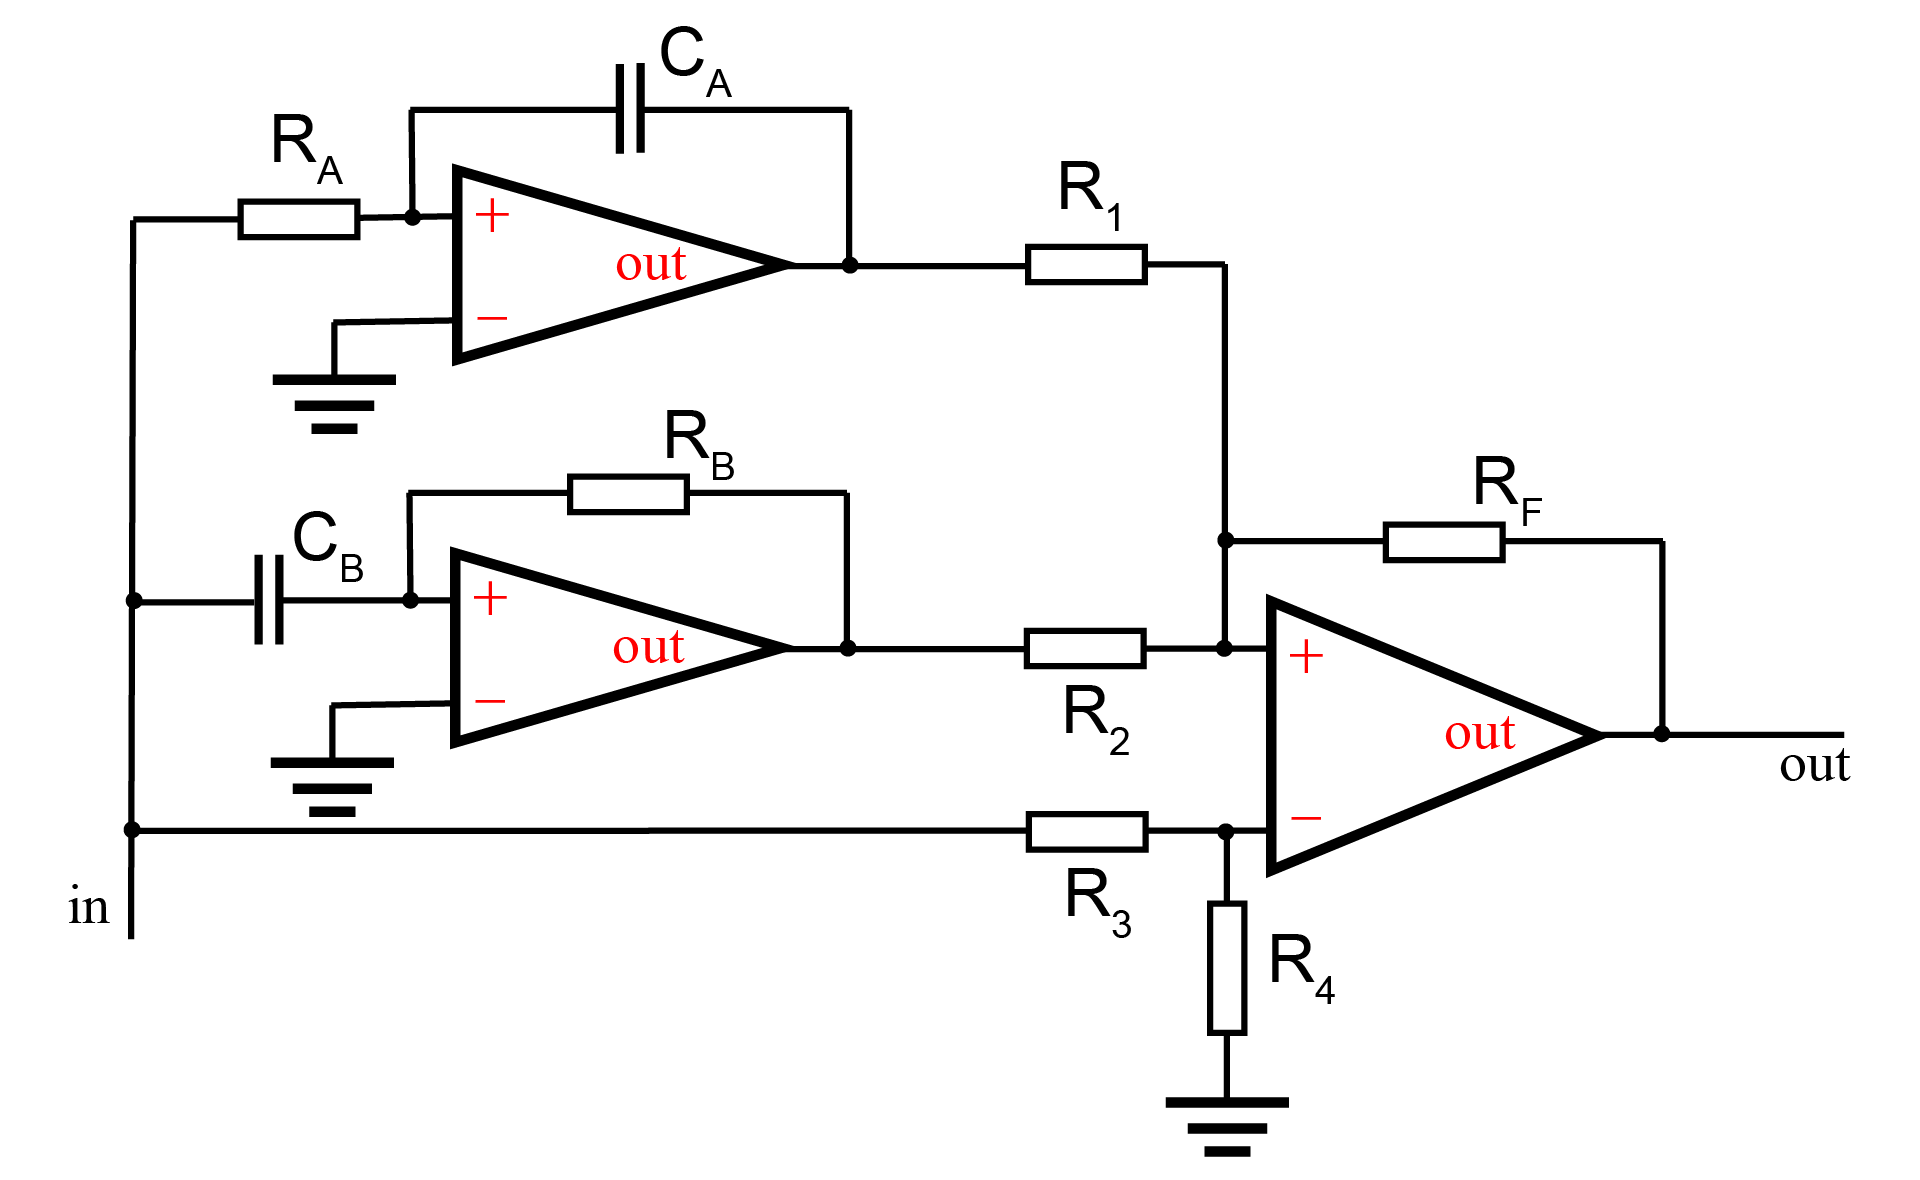
\includegraphics[width=0.7\columnwidth]{FB.png}
	\end{figure}
	
	根据电路,联立\eqref{E6-29}\eqref{E6-31}\eqref{E6-33},得到
	\begin{equation}
		u_U(t)=\frac{R_F}{R_1C_AR_A}\int_0^t u_E(t')\ud t'+\frac{R_FC_BR_B}{R_2}\frac{\ud u_E(t)}{\ud t}+\left(1+\frac{R_F(R_1+R_2)}{R_1R_2}\right)\frac{R_4}{R_3+R_4}u_E(t)
	\end{equation}
	
	即
	\begin{equation}
		K_p=\left(1+\frac{R_F(R_1+R_2)}{R_1R_2}\right)\frac{R_4}{R_3+R_4},\,K_i=\frac{R_F}{R_1C_AR_A},\,K_d=\frac{R_FC_BR_B}{R_2}
	\end{equation}\\
	
	【注】特别地,上述解答不包含本题中的两个彩蛋问题(对应的分数为$2\times20\ui$)。
	
	
	
	
	
	
	
	
	
	
	
	
\end{document}